\subsection{Упражнение 1}

Измените пример в chap10.ipynb и убедитесь, что дополнение нулями устраняет лишнюю ноту в начале фрагмента:

\begin{lstlisting}[language=Python]
if not os.path.exists('180960__kleeb__gunshot.wav'):
    !wget https://github.com/AllenDowney/ThinkDSP/raw/master/code/180960__kleeb__gunshot.wav
response = read_wave('180960__kleeb__gunshot.wav')

start = 0.12
response = response.segment(start=start)
response.shift(-start)

response.normalize()
response.plot()
decorate(xlabel='Time (s)')
\end{lstlisting}
\begin{figure}[H]
	\begin{center}
		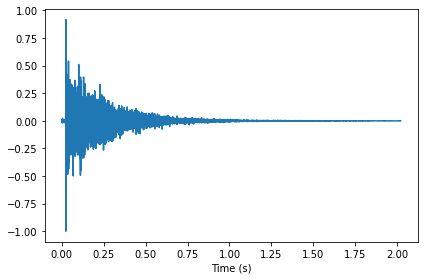
\includegraphics[scale=1]{fig/lab10/lab10_5_0.png}
		\caption{Сигнал}
	\end{center}
\end{figure}

\begin{lstlisting}[language=Python]
transfer = response.make_spectrum()
transfer.plot()
decorate(xlabel='Frequency (Hz)', ylabel='Amplitude')
\end{lstlisting}
\begin{figure}[H]
	\begin{center}
		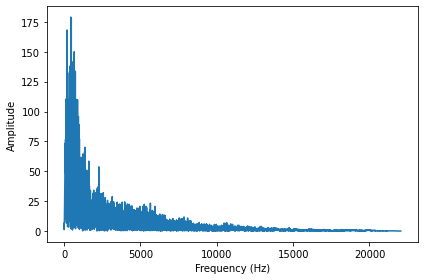
\includegraphics[scale=1]{fig/lab10/lab10_7_0.png}
		\caption{Спектр сигнала}
	\end{center}
\end{figure}

Теперь перейдём к самой записе:

\begin{lstlisting}[language=Python]
if not os.path.exists('92002__jcveliz__violin-origional.wav'):
    !wget https://github.com/AllenDowney/ThinkDSP/raw/master/code/92002__jcveliz__violin-origional.wav
    
violin = read_wave('92002__jcveliz__violin-origional.wav')

start = 0.11
violin = violin.segment(start=start)
violin.shift(-start)

violin.truncate(len(response))
violin.normalize()
violin.plot()
decorate(xlabel='Time (s)')
\end{lstlisting}
\begin{figure}[H]
	\begin{center}
		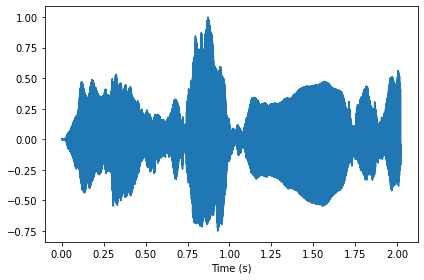
\includegraphics[scale=1]{fig/lab10/lab10_9_0.png}
		\caption{График сигнала}
	\end{center}
\end{figure}

Произведём умножения спектров и посмотрим на результат:

\begin{lstlisting}[language=Python]
spectrum = violin.make_spectrum()
wave = (spectrum * transfer).make_wave()
wave.normalize()
wave.plot()
\end{lstlisting}
\begin{figure}[H]
	\begin{center}
		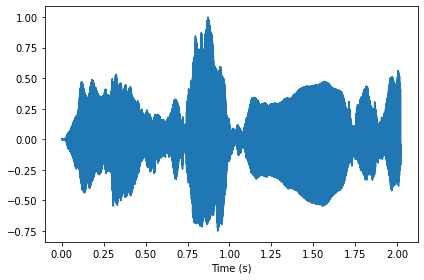
\includegraphics[scale=1]{fig/lab10/lab10_9_0.png}
		\caption{График получившегося сигнала}
	\end{center}
\end{figure}

Проблема с нотой решена.

\subsection{Упражнение 2}

Смоделируйте двумя способами звучание записи в том пространстве, где была измерена импульсная харпактеристика, как свёрткой самой записи с импульсной характеристикой, так и умножением ДПФ записи на вычисленный фильтр, соотвествующий импульсной характеристики.

\noindent Я взял себе такую характеристику: https://www.openair.hosted.york.ac.uk/?page\_id=745, а потом ничего не заработало и на выходе был дикий шум, так что я взял характеристику из учебника:

\begin{lstlisting}[language=Python]
if not os.path.exists('stalbans_a_mono.wav'):
    !wget https://github.com/AllenDowney/ThinkDSP/raw/master/code/stalbans_a_mono.wav

response = read_wave('stalbans_a_mono.wav')

start = 0
duration = 5
response = response.segment(duration=duration)
response.shift(-start)

response.normalize()
response.plot()
decorate(xlabel='Time (s)')
decorate(xlabel='Time (s)')
\end{lstlisting}
\begin{figure}[H]
	\begin{center}
		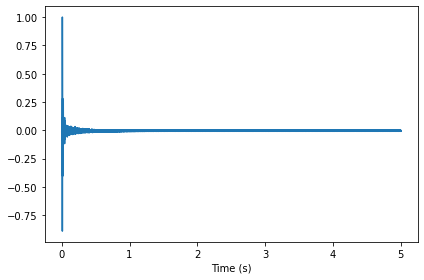
\includegraphics[scale=1]{fig/lab10/lab10_18_0.png}
		\caption{График загруженного сигнала}
	\end{center}
\end{figure}

\begin{lstlisting}[language=Python]
transfer = response.make_spectrum()
transfer.plot()
decorate(xlabel='Frequency (Hz)', ylabel='Amplitude')
\end{lstlisting}
\begin{figure}[H]
	\begin{center}
		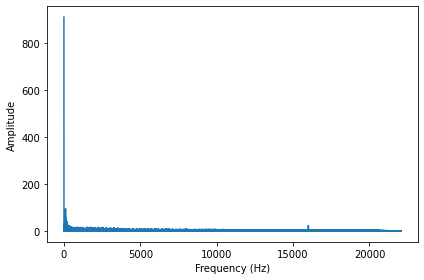
\includegraphics[scale=1]{fig/lab10/lab10_21_0.png}
		\caption{ДПФ импульсной характеристики}
	\end{center}
\end{figure}

Теперь самое интересное, промоделируем запись в пространстве.

\begin{lstlisting}[language=Python]
if not os.path.exists('164718__bradovic__piano.wav'):
    !wget https://github.com/wooftown/spbstu-telecom/raw/main/Content/164718__bradovic__piano.wav
    
wave = read_wave('164718__bradovic__piano.wav')

start = 0.0
wave = wave.segment(start=start)
wave.shift(-start)

wave.truncate(len(response))
wave.normalize()
wave.plot()
decorate(xlabel='Time (s)')
\end{lstlisting}
\begin{figure}[H]
	\begin{center}
		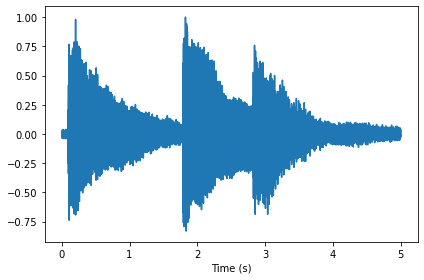
\includegraphics[scale=1]{fig/lab10/lab10_24_0.png}
		\caption{Сигнал звука пианино}
	\end{center}
\end{figure}

С использованием свёртки:
\begin{lstlisting}[language=Python]
convolved2 = wave.convolve(response)
convolved2.normalize()
convolved2.make_audio()
\end{lstlisting}

Через умножение:
\begin{lstlisting}[language=Python]
out_wave = (spectrum * transfer).make_wave()
out_wave.normalize()
out_wave.plot()
\end{lstlisting}

В результате мы добились желаемой цели.


\subsection{Вывод}

В данной работе были рассмотренны основные позиции из теории сигналов и систем. Как примеры - музыкальная акустика. При описании линейных стационарных систем используется теорема о свёртке.